\section{Flottabilité et principe d’Archimède}

\begin{frame}{Principe d’Archimède}
  \begin{block}{Énoncé}
    Tout corps plongé dans un fluide subit une \textbf{poussée verticale de bas en haut}
    égale au \textbf{poids du volume de fluide déplacé}.
  \end{block}

  \begin{itemize}
    \item Deux forces s’opposent :
          \begin{itemize}
            \item le \textbf{poids réel} du plongeur + équipement,
            \item la \textbf{poussée d’Archimède}.
          \end{itemize}
    \item Poids apparent :
          \[
            P_{\text{app}} = P_{\text{réel}} - \text{poussée d’Archimède}
          \]
  \end{itemize}
\end{frame}

\begin{frame}{Exemple de flottabilité}
  \begin{columns}[c]
    \begin{column}{0.6\textwidth}
    \begin{itemize}
      \item Corps de volume 2 L, poids réel 1 kg.
      \item Dans l’eau : volume d’eau déplacé = 2 L $\Rightarrow 2$ kg.
      \item Poids apparent : $1 - 2 = -1$ kg $\Rightarrow$ le corps \textbf{flotte}.
    \end{itemize}

    \begin{block}{Interprétation}
      \begin{itemize}
        \item Poids apparent \textbf{négatif} : flottant.
        \item Poids apparent \textbf{positif} : coule.
        \item Poids apparent \textbf{nul} : équilibre (flottabilité neutre).
      \end{itemize}
    \end{block}
    \end{column}
    \begin{column}{0.4\textwidth}
      \centering
      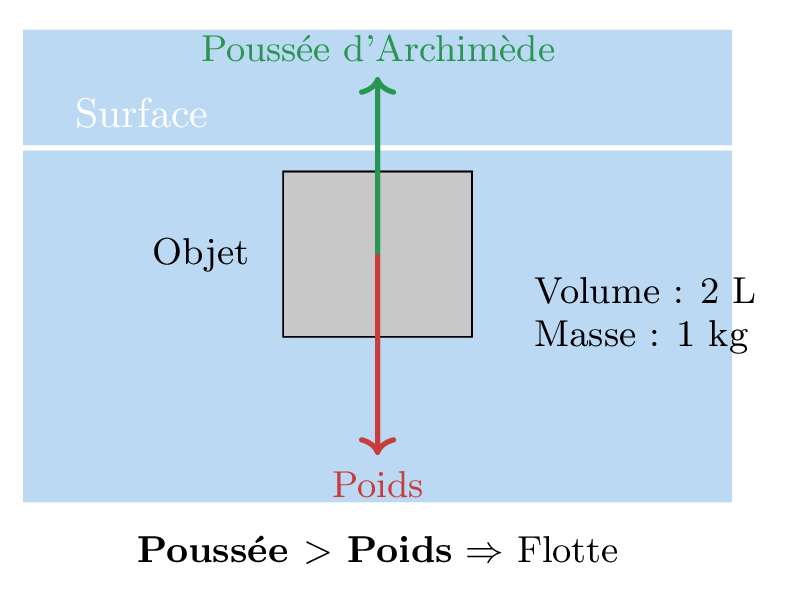
\includegraphics[height=0.5\textheight]{images/flottabilite_archimede}
    \end{column}
  \end{columns}
\end{frame}

\begin{frame}{Application au plongeur}
  \begin{itemize}
    \item Utiliser les \textbf{poumons comme ballast} (inspiration / expiration).
    \item Avoir un \textbf{lestage adapté} à sa morphologie et à l’équipement.
    \item Utiliser un \textbf{gilet stabilisateur} adapté et en bon état.
    \item Objectif : \textbf{flottabilité neutre} en plongée, confortable et sécurisante.
  \end{itemize}
\end{frame}
